\newcommand{\RLN}{ROLE}
\newcommand{\hs}{\hspace{1mm}}
\renewcommand{\t}[1]{{\mathtt{#1}}}
\renewcommand{\r}[1]{{\mathrm{#1}}}
\renewcommand{\b}[1]{{\mathbf{#1}}}
\renewcommand{\c}[1]{{\mathcal{#1}}}
\newcommand{\rR}{\r{R}}
\newcommand{\rF}{\r{F}}
\newcommand{\bW}{{\mathbb{W}}}
\newcommand{\bU}{{\mathbb{U}}}
\newcommand{\rTarg}{r_{2^\r{ce}\mhyphen\r{arg}}}
\newcommand{\SCANnet}{SCAN-net}
\newcommand{\hi}[1]{{\color{blue} #1}}
\newcommand{\add}[1]{{\textbf{\color{blue} #1}}}
\newcommand{\del}[1]{{\textbf{\color{orange} #1}}}

\chapter{Discovering the Compositional Structure of Vector Representations with Role Learning Networks} \label{chap:chap-1}

\begin{singlespace}         % you can also use `onehalfspace` to relax the spacing
    This chapter is reprinted from \fullcite{soulos-etal-2020-discovering}. Licensed under CC BY 4.0.
\end{singlespace} 

%% add your chapter text here

\begin{abstract}
    How can neural networks perform so well on compositional tasks even though they lack explicit compositional representations?
    We use a novel analysis technique called ROLE to show that recurrent neural networks perform well on such tasks by converging to solutions which implicitly represent symbolic structure. This method uncovers a symbolic structure which, when properly embedded in vector space, closely approximates the encodings of a standard seq2seq network trained to perform the compositional SCAN task. We verify the causal importance of the discovered symbolic structure by showing that, when we systematically manipulate hidden embeddings based on this symbolic structure, the model's output is changed in the way predicted by our analysis.
\end{abstract}

\section{Introduction} \label{sec:Intro}

\begin{figure}
    \footnotesize
    
    \definecolor{myblue}{RGB}{255,255,255}
    \definecolor{mybluebox}{RGB}{64,64,64}
    
    \begin{tcolorbox}[width=.5\columnwidth, colback={myblue}, coltitle=white, toptitle=3pt, bottomtitle=3pt, colframe={mybluebox},outer arc=2mm,colupper=black, valign=center, halign=left, boxsep = 0pt, title={\textbf{Goal: Interpret neural network encodings}}, halign title=center, segmentation style={solid, line width=1pt}, left=0pt]
            \def\arraystretch{1.0}% 
    
        \includegraphics[width=.5\columnwidth]{images/rldn/rolefig_top.pdf}
        \end{tcolorbox}
        
        \hypersetup{linkcolor=white}
        
        \begin{tcolorbox}[width=.5\columnwidth, colback={myblue}, coltitle=white, toptitle=3pt, bottomtitle=3pt, colframe={mybluebox},outer arc=2mm,colupper=black, valign=center, halign=left, boxsep = 0pt, title={\textbf{Method: Approximate the encodings of a neural network with a more \\ interpretable compositional model}  (\S \color{white}\ref{sec:Role-Learning})}, halign title=center, segmentation style={solid, line width=1pt}, left=3pt]
            \def\arraystretch{1.0}% 
        
        \textbf{Step 1: Assign structural roles to words using a learned role assigner.} 
        %(\S \ref{sec:Role-Learning})
        
        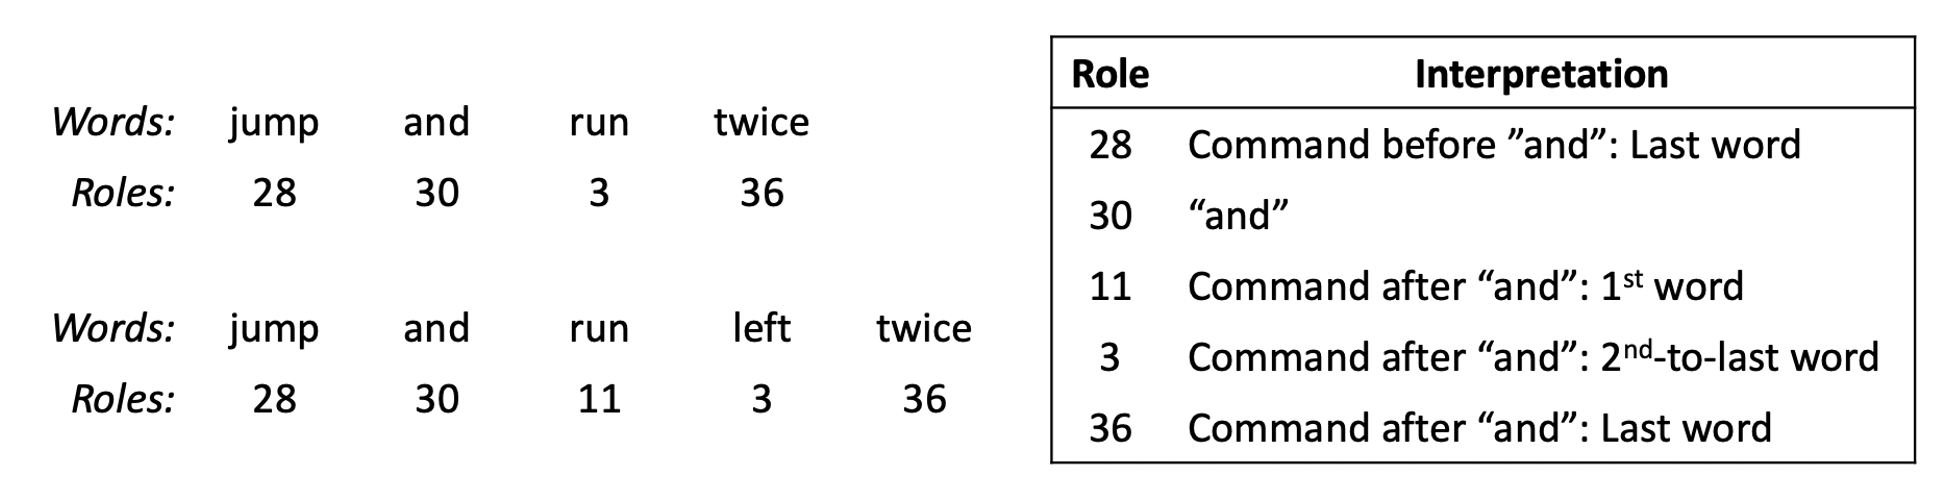
\includegraphics[width=.5\columnwidth]{images/rldn/rolefig2.png}
        
       \textbf{Step 2: Combine word and role vectors using a closed-form equation with learned parameters.} 
     %   {\scriptsize (\S \ref{sec:SCANnetReps})}
        
        \includegraphics[width=.5\columnwidth]{images/rldn/rolefig_middle.pdf}
        
         \end{tcolorbox}
        
        \hypersetup{linkcolor=blue}
        
        \begin{tcolorbox}[width=.5\columnwidth, colback={myblue}, coltitle=white, toptitle=3pt, bottomtitle=3pt, colframe={mybluebox},outer arc=2mm,colupper=black, valign=center, halign=left, boxsep = 0pt, title={\textbf{Results:}}, halign title=center, segmentation style={solid, line width=1pt}, left=3pt]
            \def\arraystretch{1.0}% 
            
        \textbf{The compositional encodings are functionally equivalent to the RNN encodings.} (\S \ref{sec:SCANnetReps})
    
        \includegraphics[width=.5\columnwidth]{images/rldn/rolefig_bottom1.pdf}
            
        \textbf{The RNN encodings can be manipulated in symbolic ways to alter the output.} (\S \ref{sec:Surgery})
        
        \includegraphics[width=.5\columnwidth]{images/rldn/rolefig_bottom2.pdf}
        
        \end{tcolorbox}
        
        \caption{Summary of our approach.}
        \label{fig:my_label}
    \end{figure}

Traditional models of cognition, and language in particular, have relied heavily on symbol structures and symbol manipulation.
However, in the current era, deep learning research has shown that Neural Networks (NNs) can display remarkable degrees of generalization on tasks traditionally viewed as depending on symbolic structure  \citep{googlenmt, mccoy}, albeit with some important limits to their generalization \citep{lake2018generalization}.
Given that standard NNs have no obvious mechanisms for representing symbolic structures, parsing inputs into such structures, nor applying compositional symbol-manipulating rules to them, this success raises the question that we address in this paper:\textbf{\emph{ How do NNs achieve such strong performance on compositional tasks?}} 

Could it be that NNs \textit{do} learn symbolic representations---covertly embedded as vectors in their state spaces?
\citet{mccoy} showed that 
when trained on highly compositional tasks, 
standard NNs learned representations that are functionally equivalent to compositional vector embeddings of symbolic structures (Sec. \ref{sec:TPR}). Processing in these NNs assigns structural representations to inputs and generates outputs that are governed by compositional rules stated over those representations. We refer to the networks we will analyze as \newterm{target NNs}, because we will propose a new type of NN (in Sec.~\ref{sec:Role-Learning})---the \newterm{Role Learner (\RLN)}---which is used to \textit{analyze} the target network.
%, after first discussing related analysis methods %of network analysis 
%in Sec.~\ref{sec:Related}.
In contrast with the analysis model of \citet{mccoy}, which relies on a hand-specified hypothesis about the structure underlying the learned representations of the target NN, \RLN\ \textit{automatically} learns a symbolic structure that best approximates the internal representation of the target network. This yields 
%Automating the discovery of structural hypotheses provides 
two %distinct 
advantages. 
First, \RLN\ achieves success at analyzing networks for which the underlying structure is unclear. We show this in Sec.~\ref{sec:SCAN}, where \RLN\ successfully uncovers the symbolic structures learned by a seq2seq RNN trained on the SCAN synthetic semantic parsing task \citep{lake2018generalization}. Second, removing the need for hand-specified structural hypotheses reduces the burden on the analyst, who only needs to provide input sequences and their target NN encodings. Discovering symbolic structure within a model enables us to perform precise alterations to the internal representations in order to produce desired alterations in the output (Sec.~\ref{sec:Surgery}). Then, in Sec.~\ref{sec:NLP}, we turn briefly to partially-compositional tasks in NLP.

The novel contributions of this research are:
\begin{itemize}
  \vspace{-2mm}
  \item ROLE, a NN module that learns to assign symbolic structures to input sequences (Sec.~\ref{sec:Role-Learning}).
  \vspace{-2mm}
  \item Demonstration that RNNs converge to compositional solutions on the synthetic SCAN task (Sec.~\ref{sec:SCAN}).
  \vspace{-2mm}
  \item A precise closed-form expression for the distributed encoding learned by an RNN trained on SCAN, exhibiting its latent symbolic structure (Sec.~\ref{sec:scan-role-interpretation}).
  \vspace{-2mm}
  \item Demonstration of the causal relevance of this symbolic structure by using the equation for its vector encoding to control RNN output through precise alteration of the RNN's internal encoding (Sec.~\ref{sec:Surgery}).
  \vspace{-2mm}
  \item Additional evidence showing that sentence embedding models do not capture compositional structure (Sec. \ref{sec:NLP}).
\end{itemize}

\section{Background Related work} \label{sec:Related}

\subsection{Compositionality}

Certain cognitive tasks consist in computing a function $\varphi$ that is governed by strict rules: e.g., if $\varphi$ is the function mapping a mathematical expression to its value (e.g., mapping `$19 - 2 * 7$' to $5$), then $\varphi$ obeys the rule that $\varphi(x + y) = \mathtt{sum}(\varphi(x), \varphi(y))$ for any expressions $x$ and $y$.
This rule is \newterm{compositional}: the output of a structure (here, $x + y$) is a function of the outputs of the structure's constituents (here, $x$ and $y$). The rule can be stated with full generality once the input is assigned a \newterm{symbolic structure} giving its decomposition into constituents. 
For a \newterm{fully-compositional} task, completely determined by compositional rules, a system that can assign appropriate symbolic structures to inputs and apply appropriate compositional rules to these structures will display full \newterm{systematic generalization}: it will correctly process arbitrary novel combinations of familiar constituents. This is a core capability of symbolic AI systems.

Other tasks, including most natural language tasks such as machine translation, are only partially characterizable by compositional rules: natural language is only partially compositional in nature. For example, if $\varphi$ is the function that assigns meanings to English adjectives, it generally obeys the rule that $\varphi(\mathtt{in\mbox{-}} + x) = \mathtt{not} \hs \varphi(x)$, (e.g., $\varphi(\mathtt{inoffensive}) = \mathtt{not} \hs \varphi(\mathtt{offensive})$), yet there are exceptions: $\varphi(\mathtt{inflammable}) = \varphi(\mathtt{flammable})$. On these ``\newterm{partially-compositional}'' tasks, this strategy of compositional analysis has demonstrated considerable, but limited, generalization capabilities.

\subsection{Analysis of NNs}

Many past works in the rich body of literature about analyzing NNs focus on compositional structure
%Our work falls within the larger paradigm of using analysis techniques to interpret NNs (see \citet{belinkov2019analysis} for a recent survey), often including a focus on compositional structure 
\citep{hupkes2020compositionality, hupkes2018visualisation, hewitt2019structural, li-etal-2019-compositional} and systematicity \citep{lake2018generalization,goodwin2020probing}. % NEW CONTENT (added "and systematicity")
Two of the most popular analysis techniques are the behavioral and probing approaches. In the behavioral approach, a model is evaluated  on a set of examples carefully chosen to require competence in particular linguistic phenomena \citep{marvin2018targeted, wang2018glue, dasgupta2019analyzing, poliak2018collecting,linzen2016assessing,mccoy2019right,warstadt2019blimp}. This technique can illuminate behavioral shortcomings but says little about how the internal representations are structured, treating the model as a black box.

In the probing approach, an auxiliary classifier is trained to classify the model's internal representations based on some linguistically-relevant distinction \citep{adi2016fine,giulianelli2018hood,conneau2018cram,conneau2018senteval,belinkov2017evaluating,blevins2018hierarchical,peters2018dissecting,tenney2018what}. In contrast with the behavioral approach, the probing approach tests whether some particular information is present in the model's encodings, but it says little about whether this information is actually used by the model. Indeed, in some cases models fail despite having the necessary information to succeed in their representations, showing that the ability of a classifier to extract that information does not mean that the model is using it \citep{ Voita2020InformationTheoreticPW, ravichander2020probing,vanmassenhove2017investigating}.

We build on \citet{mccoy}, which introduced the analysis task \newterm{DISCOVER (DISsecting COmpositionality in VEctor Representations)}:  take a NN and, to the extent possible, find an explicitly-compositional approximation to its internal distributed representations. DISCOVER allows us to bridge the gap between representation and behavior: It reveals not only what information is encoded in the representation, but also reveals this information in a way that we can manipulate to show that the information is causally implicated in the model's behavior (Section~\ref{sec:Surgery}). Moreover, it provides a much more comprehensive window into the representation than the probing approach does; while probing extracts particular types of information from a representation (e.g., ``does this representation distinguish between active and passive sentences?''), DISCOVER exhaustively decomposes the model's representational space. In this regard, DISCOVER is most closely related to the approaches of \citet{andreas2019measuring}, \citet{chrupala2019correlating}, and \citet{abnar2019blackbox}, who also propose methods for discovering a complete symbolic characterization of a set of vector representations, and \citet{omlin1996extraction} and \citet{weiss2018extracting}, which also seek to extract  more interpretable symbolic models that approximate neural network behavior.
Like \citet{andreas2019measuring} and \citet{chrupala2019correlating}, we seek to find the structure encoded in neural networks, rather than seeking structure directly from the data as is the goal in grammar induction work such as \citet{shen2018ordered} and \citet{bowman2016fast}.

\section{NN embedding of symbol structures} \label{sec:TPR}

\citeauthor{mccoy} showed that, in GRU \citep{cho-etal-2014-learning} encoder-decoder networks performing simple, fully-compositional string manipulations, the medial encoding (between encoder and decoder) could be extremely well approximated, up to an affine transformation, by \newterm{Tensor Product Representations (TPRs)} \citep{Smolensky:1990:TPV:102418.102425}, which are explicitly-compositional vector embeddings of symbolic structures. To represent a string of symbols as a TPR, the symbols in the string $\t{337}$ might be parsed into three constituents $\{ \t{3}\colon\!\r{pos}1, \t{7}\colon\!\r{pos}3, \t{3}\colon\!\r{pos}2 \}$, where $\r{pos}n$ is the role of $n^{\r{th}}$ position from the left edge of the string; other role schemes are also possible, such as roles denoting right-to-left position: $\{ \t{3}\colon\!\r{third\mbox{-}to\mbox{-}last}, \t{3}\colon\!\r{second\mbox{-}to\mbox{-}last}, \t{7}\colon\!\r{last} \}$. The embedding of a constituent $\t{7}\colon\!\r{pos}3$ is $\b{e}(\t{7}\colon\!\r{pos}3) = \b{e}_\rF(\t{7}) \otimes \b{e}_\rR(\r{pos3})$, where $\otimes$ is the tensor product (outer product), $\b{e}_\rR, \b{e}_\rF$ are respectively a vector embedding of the roles and a vector embedding of the \newterm{fillers} of those roles: the digits. The embedding of the whole string is the sum of the embeddings of its constituents. 
In general, for a symbol structure $\t{S}$ with roles $\{ r_k \}$ that are respectively filled by the symbols $\{ \t{f}_k \}$,
$\b{e}_\r{TPR}(\t{S}) = \sum_k \b{e}_\rF(\t{f}_k) \otimes \b{e}_\rR(r_k)$. The DISCOVER task including the TPR equations is depicted in Figure \ref{fig:discover}.

\begin{figure}[t]
    \centering
    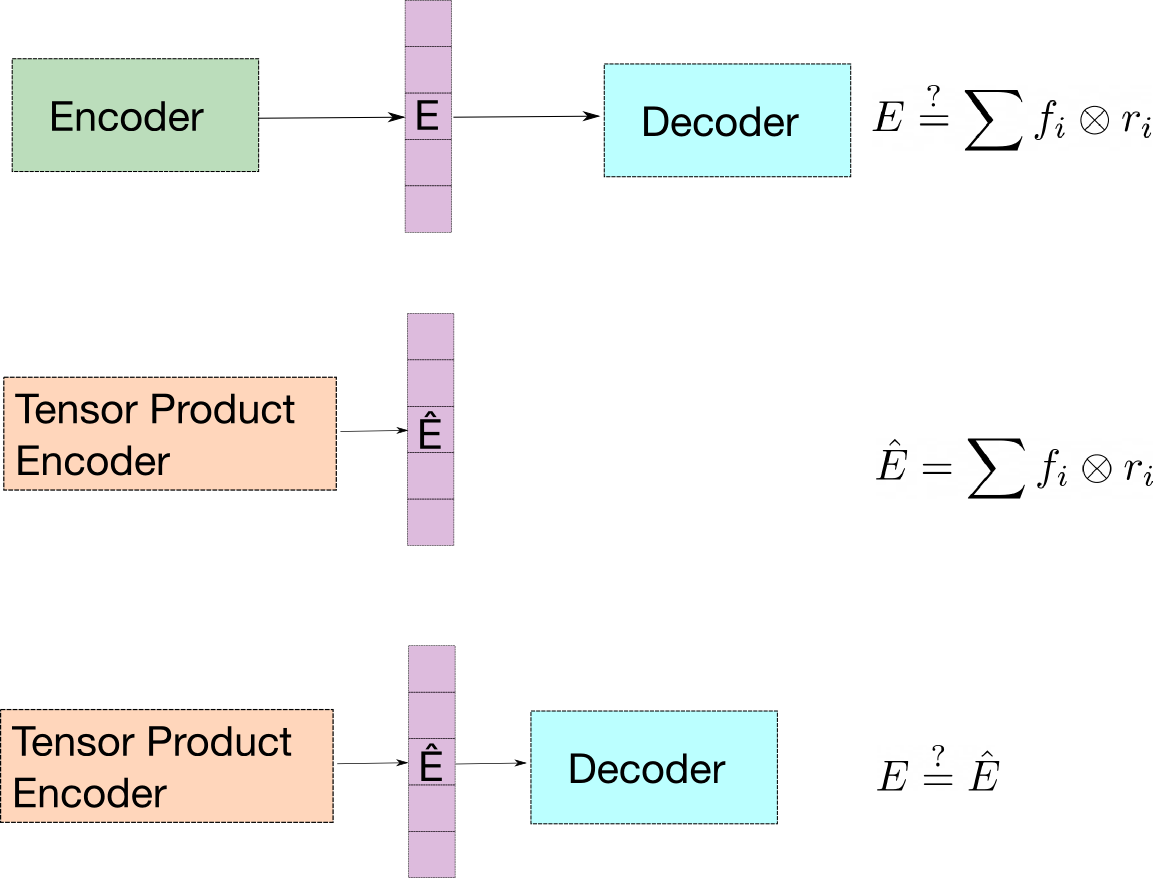
\includegraphics[scale=.25]{images/rldn/task.png}
    \caption{The DISCOVER task and functions. At the top is the target network and question we pose: is the internal embedding a TPR? The middle row is the TPE which follows the provided equation. We train the TPE to minimize the MSE between $\hat{E}$ and $E$. In the bottom row, we evaluate our model by passing the approximations $\hat{E}$ through the decoder and checking the \textit{substitution accuracy} --- the proportion of examples for which the approximated encoding $\hat{E}$ yields the correct output when provided to the decoder .}
    \label{fig:discover}
\end{figure}

At a high level, these role embeddings serve a similar purpose as positional embeddings in a Transformer \citep{vaswani2017attention}, in that they are vector embeddings of a token's position in a sequence. The roles discussed above---and the positional embeddings used in Transformers---illustrate \textbf{role schemes} based on sequential position; non-sequential role schemes such as positions in a tree are also possible. \citet{mccoy} showed that,for a given seq2seq architecture learning a given string-mapping task, there exists a highly accurate TPR approximation of the medial encoding, given an appropriate  pre-defined role scheme. The main technical contribution of the present paper is the Role Learner (ROLE) model, an RNN that learns its own role scheme to optimize the fit of a TPR approximation to a given set of internal representations in a pre-trained target NN. This makes the DISCOVER framework more general by removing the need for human-generated hypotheses about the role schemes the network might be implementing. Learned role schemes, we will see in Sec.~\ref{sec:SCANnetReps}, can enable good TPR approximation of networks for which human-generated role schemes fail.

\section{The Role Learner (ROLE) Model} \label{sec:Role-Learning} 

\RLN\footnote{Code available at \url{https://github.com/psoulos/role-decomposition}.} produces a vector-space embedding of an input string of $T$ symbols $\t{S} = \t{s}_1 \t{s}_2 \ldots \t{s}_T$ by producing a TPR $\b{T}(\t{S})$ and then passing it through an affine transformation.
%$\bW$.
\RLN\ is trained to approximate a pre-trained target string-encoder $\c{E}$.
Given a set of $N$ training strings $\{ \t{S}^{(1)}, \ldots, \t{S}^{(N)} \}$, \RLN\ minimizes the total mean-squared error (MSE) between its output $\bW\,\b{T}(\t{S}^{(i)}) + \vb$ and %$\c{E}$'s corresponding output, 
$\c{E}(\t{S}^{(i)})$.

\begin{figure}[t]
    \centering
    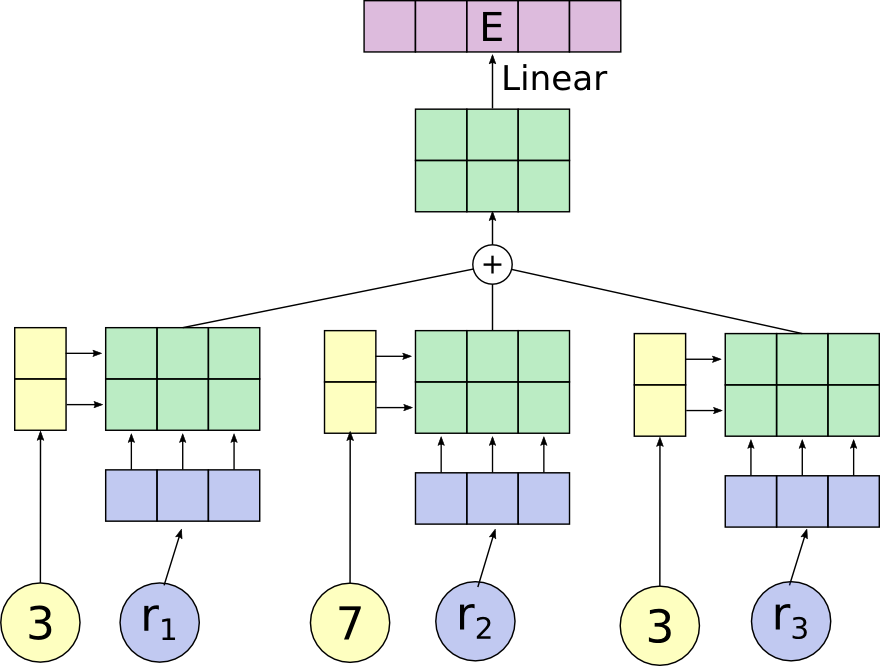
\includegraphics[scale=.3]{images/rldn/tpdn.png}
    \caption{The Tensor Product Encoder architecture. The fillers (yellow circles) and roles (blue circles) are first vectorized with an embedding layer. These two vector embeddings are combined by an outer product to produce the green matrix representing the TPR of the constituent. All of the constituents are summed together to produce the TPR of the sequence, and then a linear transformation is applied to resize the TPR to the target encoder's dimensionality. \RLN\ replaces the role embedding layer and directly produces the blue role vector.}
    \label{fig:tpe-arch}
\end{figure}

\RLN\ is an extension of the Tensor-Product Encoder (TPE) introduced in \citet{mccoy} (as the ``Tensor Product Decomposition Network'') and depicted in Figure \ref{fig:tpe-arch}. 
Crucially, \RLN\ is not \textit{given} role labels for the input symbols, but \textit{learns to compute} them.
More precisely, it learns a dictionary of $n_\rR$ $d_\rR$-dimensional role-embedding vectors, 
$\mR \in \R^{d_\rR \times n_\rR}$, and, for each input symbol 
$\t{s}_t$, computes a soft-attention vector $\va_t$ over these role vectors: 
the role vector assigned to $\t{s}_t$ is then the attention-weighted linear combination of role vectors, $\vr_t = \mR\, \va_t$. \RLN\ simultaneously learns a dictionary of $n_\rF$ $d_\rF$-dimensional symbol-embedding filler vectors $\mF \in \R^{d_\rF \times n_\rF}$, the $\phi^{\r{th}}$ column of which is $\vf_\phi$, the embedding of symbol type $\phi$; $\phi \in 1, \ldots, n_\rF$ where $n_\rF$ is the size of the vocabulary of symbol types.
The TPR generated by \RLN\ is thus $\b{T}(\t{S}) = \sum_{t=1}^T \vf_{\tau(\t{s}_t)} \otimes \vr_t$, where $\tau(\t{s}_t)$ is symbol $\t{s}_t$'s type.
Finally, \RLN\ learns an affine transformation to map this TPR into $\R^d$, where $d$ is the dimension of the representations of the encoder $\c{E}$.
%it is learning to approximate.

\begin{figure}[t]
    \captionsetup{width=\columnwidth}
    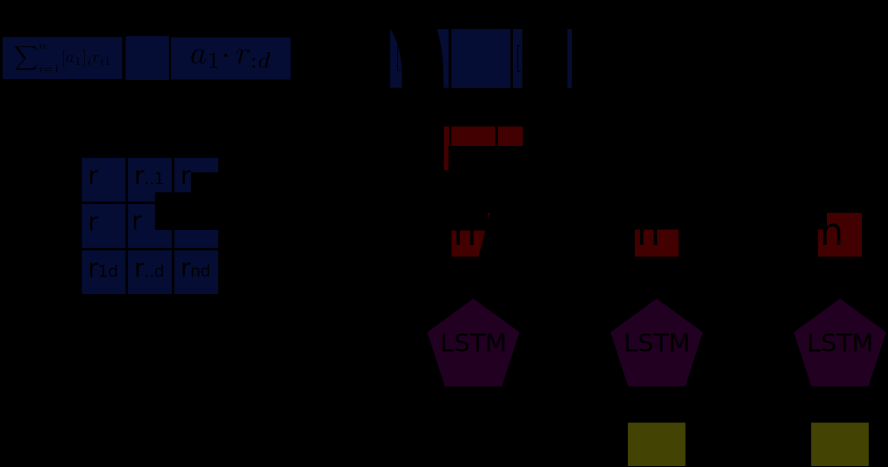
\includegraphics[width=\columnwidth]{images/rldn/role_assigner_shrink}
    \caption{The role learning module. The role attention vector $a_t$ is encouraged to be one-hot through regularization; if $a_t$ were one-hot, the produced role embedding $r_t$ would correspond directly to one of the roles defined in the role matrix $\mR$. The LSTM can be unidirectional or bidirectional.}
    \label{fig:role_learner}
\end{figure}

\RLN\ uses an LSTM \citep{Hochreiter:1997:LSM:1246443.1246450} to compute the role-assigning attention-vectors $\va_t$ from its learned embedding $\mF$ of the input symbols $\t{s}_t$: at each $t$, the hidden state of the LSTM passes through a linear layer and then a softmax to produce $\va_t$ (depicted in Figure \ref{fig:role_learner}). Let the $t^{\r{th}}$ LSTM hidden state be $\vq_t \in \R^H$; let the output-layer weight-matrix have rows $\vk_\rho^\top \in \R^H$ and let the columns of $\mR$ be $\vv_\rho \in R^{d_\rR}$, with $\rho = 1,\dots,n_\rR$. Then $\vr_t = \mR\, \va_t = \sum_{\rho=1}^{n_\rR} \vv_\rho\, \softmax ( \vk_\rho^\top \vq_t )$: the result of query-key attention  \citep[e.g.,][]{vaswani2017attention} with query $\vq_t$ to a fixed external memory containing key-value pairs $\{ ( \vk_\rho, \vv_\rho ) \}_{\rho=1}^{n_\rR}$.

Since a TPR for a discrete symbol structure deploys a discrete set of roles specifying discrete structural positions, ideally a single role would be selected for each $\t{s}_t$: $\va_t$ would be one-hot.
\RLN\ training therefore deploys regularization to bias learning towards one-hot $\va_t$ vectors (based on the regularization proposed in \citet{palangi}, developed for the same purpose). See Appendix \ref{sec:role-regulatization} for the precise regularization terms that we used.

It is essential to note that, while we impose this regularization on \RLN, there is no explicit bias favoring discrete compositional representations in the \textit{target encoder} $\c{E}$: any such structure that \RLN\ finds hidden in the representations learned by $\c{E}$ must result from biases implicit in the vanilla RNN-architecture of $\c{E}$ when applied to its target task.

\section{The SCAN task} \label{sec:SCAN}

Returning to our central question from Sec.~\ref{sec:Intro}, how can neural networks \textit{without} explicit compositional structure perform well on fully-compositional tasks? 
Our hypothesis is that, though these models have no \textit{constraint} forcing them to be compositional, they still have the \textit{ability} to implicitly learn compositional structure.
To test this hypothesis, we apply \RLN\ to a standard RNN-based seq2seq model \citep{sutskever2014sequence} trained on a fully compositional task. Because the RNN has no constraint forcing it to use TPRs, we do not know \textit{a priori} whether there exists any solution that \RLN\ could learn; thus, if \RLN\ does learn anything it will be a significant empirical finding about how these RNNs operate.

We consider the SCAN task \citep{lake2018generalization}, which was designed to test compositional generalization and systematicity. SCAN is a synthetic semantic parsing
%sequence-to-sequence mapping 
task: an input sequence describing an action plan, e.g., \textcolor{violet}{$\t{jump \hs opposite \hs left}$}, is mapped to a sequence of primitive actions, e.g., \textcolor{violet}{$\t{TL \hs TL \hs JUMP}$} (see Sec.~\ref{sec:Surgery} for a complex example). We use \textcolor{violet}{$\t{TL}$} to abbreviate \textcolor{violet}{$\t{TURN\_LEFT}$}, sometimes written \textcolor{violet}{$\t{LTURN}$}; similarly, we use \textcolor{violet}{$\t{TR}$} for \textcolor{violet}{$\t{TURN\_RIGHT}$}. The SCAN mapping is defined by a complete set of compositional rules \citep[Supplementary Fig. 7]{lake2018generalization}. 

\begin{table*}[ht]
\resizebox{\textwidth}{!}{
\begin{tabular}{ c c c c c c c c c} 
 \toprule
  \textbf{Continuous} & \textbf{Snapped} & \textbf{Discrete} & LTR & RTL & Bi & Tree & Wickel & BOW \\ 
  \midrule
  94.83\% & 81.71\% $\pm$ 7.28 & 92.44\% & 6.68\% & 6.96\% & 10.72\% & 4.31\% & 44.00\% & 4.52\% \\
 \bottomrule
\end{tabular}
}
\caption{\label{tab:scan-accuracy}Mean substitution accuracy for learned (bold) and hand-defined role schemes on SCAN across three random initializations. Standard deviation was below 1\% for all schemes except for snapped. Substitution accuracy is measured by feeding \RLN's approximation to the target decoder. (Sec.~\ref{sec:SCANnetReps})}
\end{table*}

\subsection{The compositional structure of SCAN encoder representations} \label{sec:SCANnetReps}

For our target SCAN encoder $\c{E}$, we trained a standard GRU with one hidden layer of dimension 100 for 100,000 steps (batch-size 1) with a dropout of 0.1 on the simple train-test split (hyperparameters determined by a limited search; see Appendix \ref{sec:rnn-scan}).
$\c{E}$ achieves $98.47\%$ (full-string) accuracy on the test set. Thus $\c{E}$ provides what we want: a standard RNN achieving near-perfect accuracy on a non-trivial fully compositional task.

After training, we extract the final hidden embedding from the encoder for each example in the training and test sets. These are the encodings we attempt to approximate as explicitly compositional TPRs. 
We provide \RLN\ with 50 roles to use as it wants (hyperparameters described in Appendix \ref{sec:role-scan}).
We evaluate the substitution accuracy that this learned role scheme provides in three ways. The \newterm{continuous} method tests ROLE in the same way as it was trained, with input symbol $\t{s}_t$ assigned role vector $\vr_t = \mR\, \va_t$. The continuous method does not produce a discrete set of role vectors because the linear layer that generates $a_t$ allows for continuously-valued weights. The remaining two methods test the efficacy of a truly discrete set of role vectors. First, in the \newterm{snapped} method, $\va_t$ is replaced at evaluation time by the one-hot vector $\vm_t$ singling out role $m_t = \argmax(\va_t)$: $\vr_t = \mR\, \vm_t$. This method serves the goal of enforcing the discreteness of roles, but it is expected to decrease performance because it tests ROLE in a different way than it was trained. Our final evaluation method, the \newterm{discrete} method, uses discrete roles without having such a train/test discrepancy by using a two-stage process. In the first stage, the snapped method is used to output one-hot vector roles $\vm_t$ for every symbol in the dataset. In the second stage, we train a TPE which does not learn roles but rather uses the one-hot vector $\vm_t$ as input during training. In this case, \RLN\ acts as an automatic data labeler, assigning a role to every input word.

For comparison, we also train TPEs using a variety of discrete hand-crafted role schemes: left-to-right (LTR), right-to-left (RTL), bidirectional (Bi), tree position, neighbor-based Wickelrole (Wickel), and bag-of-words (BOW) (descriptions of these role schemes are in Appendix \ref{sec:role-schemes}). 

The mean substitution accuracy from these different methods is shown in Table \ref{tab:scan-accuracy}. 
All of the predefined role schemes provide poor approximations, none surpassing $44.00\%$ accuracy. 
The role scheme learned by \RLN\ does significantly better than any of the predefined role schemes: when tested with the basic, continuous role-attention method, the accuracy is $94.83\%$. 

The success of \RLN\ 
tells us two things. First, it shows that the target model's compositional behavior relies on compositional internal representations: it was by no means guaranteed to be the case that \RLN\ would be successful here, so the fact that it is successful tells us that the encoder has learned compositional representations. Second, it adds further validation to the efficacy of \RLN, because it shows that it can be a useful analysis tool in cases of significantly greater complexity than the simple string manipulation tasks studied in \citet{mccoy}. 
In fact, it allows us to \textit{\textbf{write in closed form the embedding}} $\b{e}(\t{S})$ of an input $\t{S} = \t{s}_1\ldots\t{s}_T$ that is learned by the SCAN encoder, to an excellent degree of approximation (as measured by substitution accuracy):
$\b{e}(\t{S}) = \bW \sum_{t=1}^T \vf_{\tau(\t{s}_t)} \otimes \vr_{\rho(\t{s}_t)} + \vb$, where $\tau(\t{s}_t)$ is symbol $\t{s}_t$'s type, $\rho(\t{s}_t)$ is the role assigned to $\t{s}_t$ by the algorithm discussed next,
%given in \hl{Appendix} \ref{sec:Alg}, 
and the matrices $\bW$, $\mF = [\vf_1 \ldots \vf_{n_\rF} ]$, and $\mR = [\vr_1 \ldots \vr_{n_\rR}]$ and bias vector $\vb$ are learned by \RLN.
Note that this expression is bilinear, even though the GRU encoder that generates it includes nonlinearities.

\subsection{Interpreting the learned role scheme}\label{sec:scan-role-interpretation}

By analyzing the roles assigned by ROLE to the sequences in the SCAN training set, we created a symbolic algorithm for predicting which role will be assigned to each filler. This section covers the primary factors of the algorithm, while the entire algorithm is described in Appendix \ref{sec:Alg} and discussed at additional length in Appendix \ref{sec:AlgDisc}. Though the algorithm was created based only on sequences in the SCAN training set, it is equally successful at predicting which roles will be assigned to test sequences, exactly matching \RLN's predicted roles for 98.7\% of sequences.

%The details of this algorithm illuminate 
The algorithm illuminates how the filler-role scheme encodes information relevant to the task. First, one of the initial facts that the decoder must determine is whether the sequence is a single command, a pair of subcommands connected by \textcolor{violet}{$\t{and}$}, or a pair of subcommands connected by \textcolor{violet}{$\t{after}$}; such a determination is crucial for knowing the basic structure of the output (how many actions to perform and in what order). We have found that role 30 is used for, and only for, the filler \textcolor{violet}{$\t{and}$}, while role 17 is used in and only in sequences containing \textcolor{violet}{$\t{after}$} (usually with \textcolor{violet}{$\t{after}$} as the filler bound to role 17). Thus, the decoder can use these roles to tell which basic structure is in play: if role 30 is present, it is an \textcolor{violet}{$\t{and}$} sequence; if role 17 is present, it is an \textcolor{violet}{$\t{after}$} sequence; otherwise it is a single command.

Once the decoder has established the basic syntactic structure of the output, it must then fill in the particular actions. This can be accomplished using the remaining roles, which mainly encode absolute position within a subcommand. For example, the last word of a subcommand before \textcolor{violet}{$\t{after}$} (e.g., \textcolor{violet}{$\t{jump \hs \textbf{left} \hs after \hs walk \hs twice}$}) is always assigned role 8, while the last word of a subcommand after \textcolor{violet}{$\t{after}$} (e.g., \textcolor{violet}{$\t{jump \hs left \hs after \hs walk \hs \textbf{twice}}$}) is always assigned role 46. Therefore, once the decoder knows (based on the presence of role 17) that it is dealing with an \textcolor{violet}{$\t{after}$} sequence, it can check for the fillers bound to roles 8 and 46 to begin to figure out what the two subcommands surrounding \textcolor{violet}{$\t{after}$} look like. The identity of the last word in a subcommand is informative because that is where a cardinality (i.e., \textcolor{violet}{$\t{twice}$} or \textcolor{violet}{$\t{thrice}$}) appears if there is one. Thus, by checking what filler is at the end of a subcommand, the model can determine whether there is a cardinality present and, if so, which one.

ROLE itself does not provide an interpretation for the symbolic structure it generates, but
we have shown that this structure can be successfully interpreted by humans. By contrast, it is very difficult to interpret the continuous neuron values of RNN representations; even the rare successful cases of doing so, such as \citet{lakretz2019emergence} and \citet{mu2020compositional}, only interpret a few isolated units, while we were able to exhaustively explain the entire symbolic structure discovered by ROLE.


\begin{figure*}[ht]
    \begin{center}
    \begin{subfigure}{0.5\textwidth}
    \fontsize{7}{8}\selectfont
    $   
    \t{run}\colon\!11 \hs \t{left}\colon\!36 \hs \t{twice}\colon\!8 \hs \t{after}\colon\!43 \hs \t{jump}\colon\!10 \hs \t{opposite}\colon\!17 \hs \t{right}\colon\!4 \hs \t{thrice}\colon\!46 \rightarrow \t{\hs\hs\hs\hs\hs\hs\hs\hs}\t{TR \hs TR \hs JUMP \hs TR \hs TR \hs JUMP \hs TR \hs TR \hs JUMP \hs TL \hs RUN \hs TL \hs RUN} \leavevmode\newline -\t{run}\colon\!11 \hs +\t{look}\colon\!11 \rightarrow \leavevmode\newline \t{\hs\hs\hs\hs\hs\hs\hs\hs}\t{TR \hs TR \hs JUMP \hs TR \hs TR \hs JUMP \hs TR \hs TR \hs JUMP \hs TL \hs \hi{LOOK} \hs TL \hs \hi{LOOK}} \leavevmode\newline
    -\t{jump}\colon\!10 \hs +\t{walk}\colon\!10 \rightarrow\leavevmode\newline
    \t{\hs\hs\hs\hs\hs\hs\hs\hs}\t{TR \hs TR \hs \hi{WALK} \hs TR \hs TR \hs \hi{WALK} \hs TR \hs TR \hs \hi{WALK} \hs TL \hs LOOK \hs TL \hs LOOK} \leavevmode\newline
    -\t{left}\colon\!36 \hs +\t{right}\colon\!36 \rightarrow\leavevmode\newline
    \t{\hs\hs\hs\hs\hs\hs\hs\hs}\t{TR \hs TR \hs WALK \hs TR \hs TR \hs WALK \hs TR \hs TR \hs WALK \hs \hi{TR} \hs LOOK \hs \hi{TR} \hs LOOK} \leavevmode\newline
    -\t{twice}\colon\!8 \hs +\t{thrice}\colon\!8 \rightarrow\leavevmode\newline
    \t{\hs\hs\hs\hs\hs\hs\hs\hs}\t{TR \hs TR \hs WALK \hs TR \hs TR \hs WALK \hs TR \hs TR \hs WALK \hs TR \hs LOOK \hs } \leavevmode\newline
    \t{\hs\hs\hs\hs\hs\hs\hs\hs}\t{TR \hs LOOK \hs \hi{TR \hs LOOK}} \leavevmode\newline
    -\t{opposite}\colon\!17 \hs +\t{around}\colon\!17 \rightarrow\leavevmode\newline
    \t{\hs\hs\hs\hs\hs\hs\hs\hs}\hi{\t{TR \hs WALK \hs TR \hs WALK \hs TR \hs WALK \hs TR \hs WALK \hs TR \hs WALK \hs TR \hs WALK}} \leavevmode\newline
    \t{\hs\hs\hs\hs\hs\hs\hs\hs}\hi{\t{TR \hs WALK \hs TR \hs WALK \hs TR \hs WALK \hs TR \hs WALK \hs \hi{TR \hs WALK \hs TR \hs WALK} \hs }} \leavevmode\newline
    \t{\hs\hs\hs\hs\hs\hs\hs\hs}\t{TR \hs LOOK \hs TR \hs LOOK \hs TR \hs LOOK} \leavevmode\newline
$
        \label{fig:role-distribution}
    \end{subfigure}
    \hfill
    \begin{subfigure}{0.28\textwidth}
        \hspace{-40pt}
        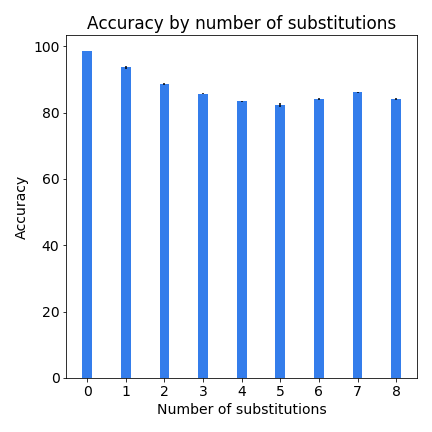
\includegraphics[width=\textwidth]{images/rldn/sub-accuracy.png}
        \label{fig:surgery}
    \end{subfigure}
    \caption{Left: Example of successive constituent surgeries. The roles assigned to the input symbols are indicated in the first line (e.g., \textcolor{violet}{$\t{run}$} was assigned role $11$). Altered output symbols are in blue. The model produces the correct outputs for all cases shown here. Right: Mean constituent-surgery accuracy across three runs. Standard deviation is below 1\% for each number of substitutions. (Sec.~\ref{sec:Surgery})}
    \label{fig:Figs12}
    \end{center}
\end{figure*}

\subsection{Precision constituent-surgery on internal representations produces desired outputs} \label{sec:Surgery}

The substitution-accuracy results above show that if the \textit{entire} learned representation is replaced by \RLN's approximation, the output remains correct. But do the \textit{individual word embeddings} in this TPR have the appropriate causal consequences when processed by the decoder?%\footnote{Historically, this question has had considerable significance: the original compositionality challenge to neural network models of cognition by Fodor and colleagues \citep{fodor1988connectionism} insisted that constituents of cognitive representations must individually be \textit{causally efficacious} in order for those constituents to provide an explanation of the compositionality of cognition \citep{fodor1990connectionism, fodor1997connectionism}. That TPRs meet the challenge of explaining compositionality was argued in \citet{smolensky1987constituent,smolensky1991connectionism}.}

To address this causal question \citep{pearl2000causality}, we actively intervene on the constituent structure of the internal representations by replacing one constituent with another syntactically equivalent
one,\footnote{We extract syntactic categories from the SCAN grammar \citep[Supplementary Fig. 6]{lake2018generalization} by saying that two words belong to the same category if every occurrence of one could be grammatically replaced by the other. We do not replace occurrences of \textcolor{violet}{$\t{and}$} and \textcolor{violet}{$\t{after}$} since the presence of either of these words causes substantial changes in the roles assigned within the sequence (Appendix \ref{sec:Alg}).} and see whether this produces the expected change in the output of the decoder.
We take the encoding generated by the RNN encoder $\c{E}$ for an input such as \textcolor{violet}{$\t{jump \hs opposite \hs left}$}, subtract the vector embedding of the \textcolor{violet}{$\t{opposite}$} constituent, add the embedding of the \textcolor{violet}{$\t{around}$} constituent, and see whether this causes the output to change from the correct output for \textcolor{violet}{$\t{jump \hs opposite \hs left}$ ($\t{TL \hs TL \hs JUMP)}$} to the correct output for \textcolor{violet}{$\t{jump \hs around \hs left}$ ($\t{TL \hs JUMP \hs TL \hs JUMP \hs TL \hs JUMP \hs TL \hs JUMP}$)}. The roles in these constituents are determined by the algorithm of Appendix \ref{sec:Alg}. If changing a word leads other roles in the sequence to change (according to the algorithm), we update the encoding with those new roles as well. Such surgery can be viewed as a more general extension of the analogy approach used by \citet{mikolov2013linguistic} for analysis of word embeddings.
An example of applying a sequence of five such constituent surgeries to a sequence is shown in Figure~\ref{fig:Figs12} (left). Even long sequences of such replacements produce the expected change in the decoder's output with high accuracy (Figure~\ref{fig:Figs12}, right), indicating that the compositional structure discovered by ROLE does play a central causal role in the model's behavior.

\section{Partially-compositional NLP tasks} \label{sec:NLP}
The previous sections explored fully-compositional tasks where there is a strong signal for compositionality. In this section, we explore whether the representations of NNs trained on tasks that are only partially-compositional also capture compositional structure. Partially-compositional tasks are especially challenging to model because a fully-compositional model may enforce compositionality too strictly to handle the non-compositional aspects of the task, while a model without a compositional bias may not learn any sort of compositionality from the weak cues in the training set.

We test four sentence encoding models for compositionality: InferSent \citep{conneau2017supervised}, Skip-thought \citep{kiros2015skip}, Stanford Sentiment Model (SST) \citep{socher2013recursive}, and SPINN \citep{bowman2016fast}. For each of these models, we extract the encodings for the SNLI premise sentences \citep{bowman2015large}. We use the extracted embeddings to train \RLN\ with 50 roles available (additional training information provided in Appendix \ref{sec:role-sentences}).

\begin{table*}[h!]
    \centering
   \resizebox{\textwidth}{!}{
		\begin{tabular} {lcccccccc}
			\toprule
		 & \textbf{Continuous} & \textbf{Snapped} & \textbf{Discrete} & LTR & RTL & Bi & Tree & BOW \\ \midrule
		InferSent & \textbf{4.05e-4} & 4.15e-4 & 5.76e-4 & 8.21e-4 & 9.70e-4 & 9.16e-4 & 7.78e-4 & 4.34e-4 \\
		Skip-thought & 9.30e-5 & 9.32e-5 & 9.85e-5 & 9.91e-5 & 1.78e-3 & 3.95e-4 & 9.64e-5 & \textbf{8.87e-5} \\
		SST & \textbf{5.58e-3} & 6.72e-3 & 6.48e-3 & 8.35e-3 & 9.29e-3 & 8.55e-3 & 5.99e-3 & 9.38e-3 \\
		SPINN & \textbf{.139} & .151 & .147 & .184 & .189 & .181 & .178 & .176 \\ \bottomrule
		\end{tabular}
		}
    \caption{\label{tab:sent-emb-mse}MSE loss for learned (bold) and hand-crafted role schemes on sentence embedding models. (Sec.~\ref{sec:NLP})}

\end{table*}

As a baseline, we also train TPEs that use pre-defined role schemes (hyperparameters described in Appendix \ref{sec:tpe-sentences}). For all of the sentence embedding models except Skip-thought, \RLN\ with continuous attention provides the lowest mean squared error at approximating the encoding (Table~\ref{tab:sent-emb-mse}). The BOW (bag-of-words) role scheme represents a TPE that uses a degenerate `compositional' structure which assigns the same role to every filler; for each of the sentence embedding models tested except for SST, performance is  within the same order of magnitude as structure-free BOW. \citet{parikh2016decomposable} found that a bag-of-words model scores extremely well on Natural Language Inference despite having no knowledge of word order, showing that structure is not necessary to perform well on the sorts of tasks commonly used to train sentence encoders. Although not definitive, the \RLN\ results provide no evidence that these models' sentence embeddings possess compositional structure.

In future work, it would be interesting to perform a similar analysis on Transformer architectures \citep{vaswani2017attention}. Such models have displayed impressive syntactic generalization \cite{hu2020systematic} and few-shot learning of compositional tasks \cite{brown2020language}, both of which suggest that they learn substantial degrees of compositional structure; thus, ROLE may be more likely to discover meaningful structure in Transformers than in the sentence-embedding models in Table \ref{tab:sent-emb-mse}. Further work has found impressive degrees of syntactic structure in Transformer encodings \cite{hewitt2019structural}, suggesting that there may well be compositional structure for ROLE to pick up on. The main difficulty in applying ROLE to Transformers---and the reason we did not include Transformers in our study---is that the sentence representation used by a Transformer is typically viewed as a variable-sized collection of vectors, whereas ROLE requires single-vector representations; this discrepancy must be overcome if ROLE is to be applied to Transformers. 

One past work \cite{jawahar-etal-2019-bert} has applied ROLE's precursor (the TPDN of \citet{mccoy}) to Transformer representations by choosing the [CLS] token of BERT \cite{devlin2019bert} as the single-vector sentence encoding to decompose. \citeauthor{jawahar-etal-2019-bert} found that these encodings were approximated better by human-specified tree-position roles than by other human-specified candidates (e.g., left-to-right and right-to-left roles). By removing the constraint of requiring human-designed role schemes, ROLE may be able to discover other role schemes that approximate BERT's encodings even more closely.
% The main difficulty in applying ROLE to Transformers---and the reason we did not include Transformers in our study---is that the sentence representation used by a Transformer is typically viewed as a variable-sized collection of vectors, whereas ROLE requires single-vector representations; this discrepancy must be overcome if ROLE is to be applied to Transformers.

\section{Conclusion} \label{sec:Conclusion}

We have introduced \RLN, a neural network that learns to approximate the representations of an existing target neural network $\c{E}$ using an explicit symbolic structure. \RLN\ successfully discovers symbolic structure in a standard RNN trained on the fully-compositional SCAN semantic parsing task, even though the RNN has no such structure explicitly present in its architecture. This yields a closed-form equation for the RNN's encoding of any input string. 
When applied to sentence embedding models trained on partially-compositional tasks, \RLN\ performs better than hand-specified hypothesized structures but still provides little evidence that the sentence encodings represent compositional structure. 

While this work has shown that NNs can converge to TPRs to solve compositional tasks, it is still unknown how the weights in the NN actually convert the raw input into a TPR. To investigate this process, in future work we plan to apply our technique to representations of partial sequences. For instance, when the complete input is \textcolor{violet}{$\t{jump \hs right \hs twice}$}, the target RNN must first represent \textcolor{violet}{$\t{jump \hs right}$} as a well-formed TPR at the point when only those two words have been encountered. The representation then needs to be updated when the next word, \textcolor{violet}{$\t{twice}$}, is encountered. By studying the nature of that update, we can gain insight into how the target model builds up a TPR from the input elements.



Uncovering the latent symbolic structure of NN representations learned for fully-compositional tasks is a significant step towards explaining how NNs achieve the level of compositional generalization that they do. In addition, by illuminating shortcomings in the representations learned for standard tasks that are not fully-compositional, ROLE can help suggest types of inductive bias for improving models' generalization with standard, partially-compositional datasets.